\documentclass[11pt,a4paper]{ctexart}

\usepackage[margin=2.6cm]{geometry}
\usepackage{amsmath,amssymb,amsthm}
\usepackage{graphicx}
\usepackage{booktabs}
\usepackage{hyperref}
\usepackage{xcolor}
\usepackage{listings}
\usepackage{caption}

\graphicspath{{figures/}}
\hypersetup{colorlinks=true, linkcolor=blue!50!black, urlcolor=blue!60!black}
\lstset{
  basicstyle=\ttfamily\small,
  breaklines=true,
  frame=single,
  columns=fullflexible,
  backgroundcolor=\color{gray!7}
}

\newtheorem{definition}{定义}[section]
\newtheorem{theorem}{定理}[section]
\newtheorem{lemma}{引理}[section]
\newtheorem{proposition}{命题}[section]
\newtheorem{example}{例}[section]

\title{第 10 章 \quad Spectral Representations / 谱表示}
\author{基于 \textit{A Course in Time Series Analysis} 的中文讲义与 Python 实践}
\date{}

\begin{document}
\maketitle

\section*{本章学习目标}

本章按照原文 \textit{Spectral Representations} 的小节顺序整理，保留主要定义、定理、模型公式和练习方向，并将原文中的 R 实践思路改写为 Python 工程实践。

完成本章后，应能够：
\begin{itemize}
  \item 回顾 DFT 在周期检测中的作用；
  \item 理解平稳序列 DFT 的近似不相关性；
  \item 掌握谱密度、谱分布和 Bochner/Herglotz 定理；
  \item 理解 Cramer 谱表示定理；
  \item 推导 MA、AR、ARMA 的谱密度。
\end{itemize}

\section{Fourier 变换的使用回顾}

前面章节已经用 DFT 找周期。对 \(X_1,\ldots,X_n\)，DFT 为
\[
  J_n(\omega)=\frac1{\sqrt n}\sum_{t=1}^n X_t e^{it\omega},
\]
周期图为 \(I_n(\omega)=|J_n(\omega)|^2\)。本章把频域工具从周期检测推广到平稳过程的完整二阶表示。

\section{DFT 的近似不相关性}

\begin{lemma}[原文 Lemma 10.2.1]
若 \(\{X_t\}\) 二阶平稳且自协方差绝对可和，则不同 Fourier 频率处的 DFT 近似不相关：
\[
  \mathrm{cov}\{J_n(\omega_j),J_n(\omega_k)\}\approx0,\qquad j\ne k.
\]
同一频率处的方差近似为谱密度。
\end{lemma}

该性质解释了为什么频域似然和 Whittle 似然可把复杂相关矩阵近似分解为频率上的独立贡献。

\section{谱表示结果概览}

频域分析的中心思想是：平稳序列的协方差函数和频率能量分布互为 Fourier 对。

\subsection{谱密度}

若 \(\sum_k|c(k)|<\infty\)，谱密度定义为
\[
  f(\omega)=\frac1{2\pi}\sum_{k=-\infty}^{\infty}c(k)e^{-ik\omega}.
\]
反演公式为
\[
  c(k)=\int_{-\pi}^{\pi}e^{ik\omega}f(\omega)\,d\omega.
\]

\begin{theorem}[谱密度非负性，原文 Theorem 10.4.1]
合法协方差序列的谱密度非负；反过来，非负可积函数通过反演公式定义合法协方差。
\end{theorem}

\section{谱分布与 Bochner 定理}

若协方差不绝对可和，也可用谱分布 \(F\) 表示：
\[
  c(k)=\int_{-\pi}^{\pi}e^{ik\omega}\,dF(\omega).
\]
\begin{theorem}[Herglotz/Bochner 定理，原文 Theorem 10.4.2]
序列 \(c(k)\) 非负定，当且仅当存在有限非负测度 \(F\)，使上述表示成立。
\end{theorem}

\section{谱表示定理}

\begin{theorem}[Cramer 谱表示，原文 Theorem 10.5.1]
零均值二阶平稳过程可写成
\[
  X_t=\int_{-\pi}^{\pi}e^{it\omega}\,dZ(\omega),
\]
其中 \(Z(\omega)\) 是正交增量过程，且增量方差由谱分布决定。
\end{theorem}

这一定理是 Wold 分解在频域中的对应物。

\section{MA、AR 和 ARMA 的谱密度}

线性过程
\[
  X_t=\sum_{j=0}^{\infty}\psi_j\varepsilon_{t-j}
\]
的谱密度为
\[
  f_X(\omega)=\frac{\sigma^2}{2\pi}
  \left|\sum_{j=0}^{\infty}\psi_je^{-ij\omega}\right|^2.
\]
ARMA(p,q) 的谱密度为
\[
  f_X(\omega)=\frac{\sigma^2}{2\pi}
  \frac{|\theta(e^{-i\omega})|^2}{|\phi(e^{-i\omega})|^2}.
\]
AR 根接近单位圆会在相应频率附近产生高谱峰。

\section{高阶谱与扩展}

原文还介绍累积量和高阶谱。二阶谱描述协方差结构，高阶谱则可捕捉非高斯和非线性依赖。缺失观测情形下，谱密度估计还需修正采样机制带来的影响。

\section{原文小节覆盖补充}

\subsection{DFT 近似不相关与平稳性检验}
第 10.2 节证明二阶平稳短记忆序列在不同 Fourier 频率上的 DFT 近似不相关。第 10.2.1 用该性质讨论二阶平稳性检验：若局部频域能量随时间变化，平稳性可能失效。Exercise 10.1 要求模拟 AR(2) 并运行相应检验。

\begin{lemma}[DFT 协方差，原文 Lemma 10.2.1--10.2.2]
若自协方差及其加权和满足可和条件，则 DFT 协方差由谱密度近似，不同 Fourier 频率之间的协方差趋于 0。
\end{lemma}

\subsection{完整去相关与谱表示总览}
第 10.2.3 解释 DFT 在理想情形下的完全去相关。第 10.3 总结 Cramer 谱表示和 Bochner/Herglotz 定理：前者表示过程本身，后者表示协方差函数。

\subsection{谱密度、谱分布和例子}
第 10.4 讨论谱密度非负性、经验协方差的谱解释、Toeplitz 方差矩阵和谱分布。纯周期成分对应谱分布跳跃，随机平稳成分对应连续谱密度。

\begin{example}[谱分布例子，原文 Example 10.4.2--10.4.3]
确定性正弦波的谱分布在对应频率处有质量点；一般平稳随机过程则通过连续谱密度分配频率能量。
\end{example}

\subsection{线性过程和 ARMA 谱密度}
第 10.6 从线性过程推出
\[
  f_X(\omega)=\frac{\sigma^2}{2\pi}|\psi(e^{-i\omega})|^2,
\]
并得到 ARMA 谱密度。Exercise 10.2 要求推导 MA(1) 谱密度。

\begin{definition}[Cramer 表示，原文 Definition 10.6.1]
线性过程可写为正交增量过程的频域积分，使滤波、谱密度和协方差反演处在统一框架内。
\end{definition}

\subsection{谱密度近似、高阶谱和附录证明}
第 10.6.3 讨论用 AR 或 MA 近似谱密度。第 10.7 引入高阶谱，第 10.8 讨论随机缺失，第 10.9 给出一般正交展开等证明。

\begin{proposition}[高阶谱，原文 Proposition 10.7.1]
若严格平稳序列具有足够高阶累积量可和性，则 q 阶谱密度定义为 q 阶累积量函数的 Fourier 变换。
\end{proposition}

\subsection{谱密度近似引理}
\begin{lemma}[原文 Lemma 10.6.1]
若 \(|c(r)|\) 可和，截断协方差对应的谱密度近似真实谱密度，误差由截断尾部控制。
\end{lemma}

\begin{lemma}[原文 Lemma 10.6.2]
若谱密度足够平滑，可用有限阶 AR 或 MA 近似其形状；该思想连接谱估计和高阶 AR 近似。
\end{lemma}

\begin{theorem}[原文 Theorem 10.9.1]
一般正交展开定理说明，不一定平稳的时间序列也可在适当正交基下展开；Cramer 表示是平稳情形的特殊版本。
\end{theorem}

\subsection{10.9 附录证明的教学作用}
原文附录的证明把谱密度非负性、谱分布构造、正交增量和一般正交展开连在一起。教学上应把它理解为三步：先由非负定协方差构造非负谱测度；再用该测度定义频域正交增量；最后用积分表示恢复时域过程。这样，Bochner 定理、Cramer 表示和 ARMA 谱密度公式就不再是孤立结论，而是同一套 Hilbert 空间投影思想在频域中的表现。

\section{Python 工程实践}

在本章目录下运行：
\begin{lstlisting}[language=bash]
python scripts/ch10_generate_figures.py
\end{lstlisting}

脚本会把图像写入本章 \texttt{figures/} 目录。当前图像用于配合本章核心概念的仿真说明；若后续补齐原始数据文件，可把模拟数据替换为原文真实数据案例。

\begin{figure}[htbp]
  \centering
  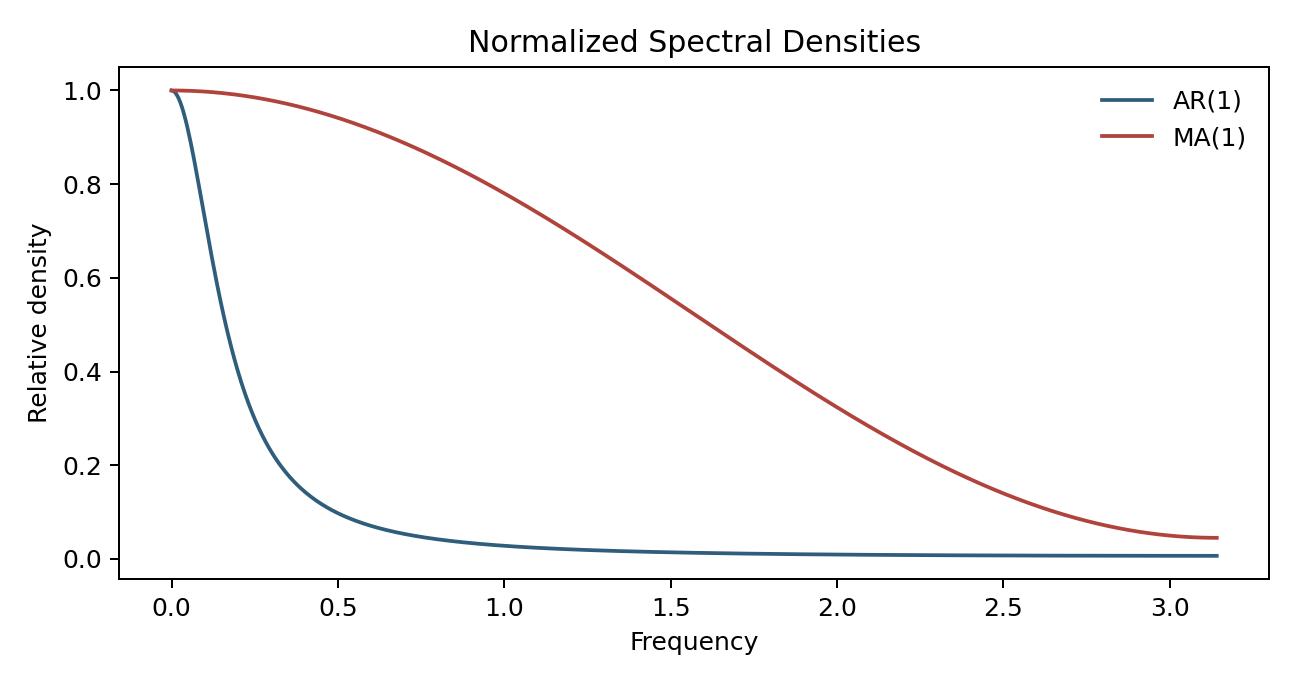
\includegraphics[width=0.86\textwidth]{ch10_fig01_spectral_density.png}
  \caption{AR 与 MA 谱密度形态：频域中不同模型表现为不同频率能量分布。}
\end{figure}

\begin{figure}[htbp]
  \centering
  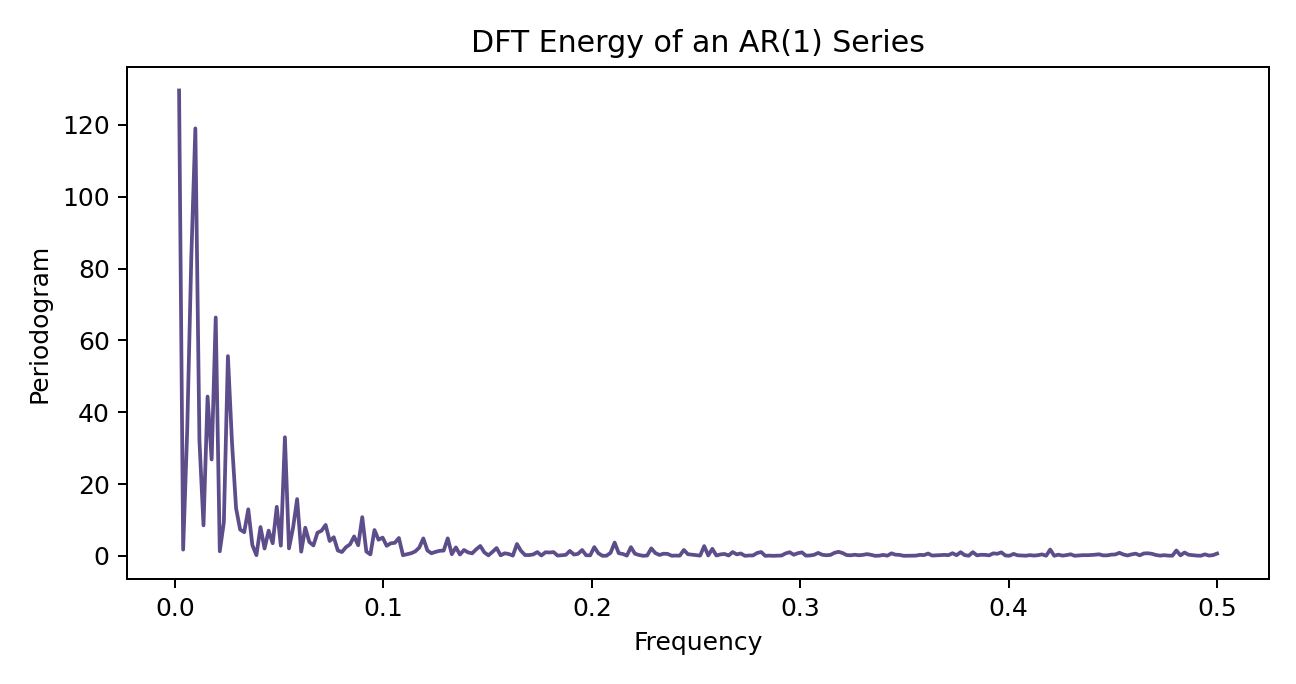
\includegraphics[width=0.86\textwidth]{ch10_fig02_dft_energy.png}
  \caption{AR(1) 序列的 DFT 能量：低频能量较强对应高持续性。}
\end{figure}

\section{练习提要}

原文练习主要围绕下列方向展开：
\begin{itemize}
  \item 推导 MA(1)、AR(1) 和 ARMA(p,q) 谱密度；
  \item 模拟 AR(2)，观察 DFT 和周期图峰值；
  \item 验证协方差和谱密度的 Fourier 反演；
  \item 阅读高阶谱定义并联系非高斯过程。
\end{itemize}

\section*{本章小结}

第 10 章给出了平稳过程的频域语言。协方差函数、谱密度和谱分布互相等价，DFT 近似去相关使频域估计成为可能，ARMA 谱密度则把模型根的位置转化为频率峰值。

\end{document}
